% Chapter 6: Work 2 Scope — LLM KV-Cache on Organic Optoelectronic CIM
% Full draft v3. Expanded from 88-line stub to ~15-page chapter draft.
% Direction: C (KV-Cache) per CLAUDE_WORK2_DIRECTION_LOCK_20260423.md
% 第六章 Work 2 范围与KV缓存评估

\chapter{大语言模型KV缓存的有机光电存内计算映射}
\label{ch:work2_scope}

\section{研究动机}
\label{sec:work2_motivation}

\subsection{大语言模型推理的存储瓶颈}

大语言模型（LLM）的能力随参数与上下文规模扩展而提升，但推理部署成本——尤其是面向终端用户的自回归解码——对延迟、吞吐和能效提出了严苛约束。

\textbf{边缘推理}（edge inference）对存储容量、计算带宽和电池能量均有严格约束。以典型智能手机为例，其可用DRAM为4–12 GB，而7B参数LLM的FP16权重即需约14 GB，加上KV缓存后远超设备容量；即使采用4-bit量化权重，KV缓存的动态增长仍可能迅速耗尽内存。

在自回归解码过程中，模型每生成一个新token，都需要计算当前token与此前所有已生成token之间的注意力（attention）分数。若采用朴素的重复计算策略，每步解码的时间复杂度为$O(n^2)$，其中$n$为已生成序列长度。为避免这一平方级开销，现代Transformer实现引入了\textbf{键值缓存（Key-Value Cache, KV缓存）}机制：在初始的预填充（prefill）阶段，模型一次性计算并存储所有输入token的Key（K）和Value（V）张量；在后续的解码（decode）阶段，只需将新生成token的K、V追加至缓存，并基于完整的K、V集合计算注意力。此举将每步解码的计算复杂度降至$O(n)$，但代价是显存占用随序列长度线性增长。

KV缓存的存储开销可量化为：
\begin{equation}
M_{\text{KV}} = 2 \times L \times H \times D_h \times S \times P
\label{eq:kv_memory}
\end{equation}
其中，$L$为Transformer层数，$H$为注意力头数，$D_h$为每头维度，$S$为当前序列长度，$P$为精度字节数（如FP16下$P=2$）。以LLaMA-2-7B为例，$L=32$，$H=32$，$D_h=128$，在上下文长度$S=4096$时，单批次FP16 KV缓存即达\textbf{2 GiB}；当扩展至32k上下文或更大批次时，KV缓存可轻松超过模型权重本身的存储 footprint。对于边缘设备（edge device）而言，如此庞大的动态存储需求已成为部署LLM的首要瓶颈。

\subsection{现有数字方案的固有折衷}

针对KV缓存的存储爆炸问题，学术界与工业界提出了四类主要缓解策略，但均在精度、延迟或系统复杂度之间存在根本性折衷。

\textbf{（1）量化压缩}。代表性工作如KIVI~\cite{liu2024kivi}提出对Key采用逐通道（per-channel）非对称量化、对Value采用逐token（per-token）非对称量化，将KV缓存压缩至2–4 bit，从而将存储开销降低4–8倍。然而，极低比特量化不可避免地引入重构误差，在长上下文场景下误差累积可导致注意力分布偏移，进而影响下游任务性能。此外，量化/反量化操作本身引入额外计算开销，在低功耗边缘场景下不可忽略。

\textbf{（2）动态驱逐}。StreamingLLM~\cite{xiao2024streamingllm}、H$_2$O~\cite{zhang2023h2o}等方法基于注意力分数的稀疏性，识别并驱逐"不重要"的历史token对应的K、V条目，以固定缓存容量上限。此类方法的局限在于：首先，注意力稀疏性分布与任务类型强相关，通用场景下难以保证稳定的精度下界；其次，驱逐决策本身需要维护辅助数据结构（如注意力汇聚池），增加了控制逻辑复杂度；最后，被驱逐的token一旦需要重新引入（如多轮对话中的指代回溯），将触发代价高昂的重新计算。

\textbf{（3）分层卸载}。InfiniGen~\cite{lee2024infinigen}、vLLM~\cite{kwon2023efficient}等系统采用CPU DRAM甚至NVMe SSD作为KV缓存的二级存储，通过精细的调度策略在GPU高带宽存储与主机大容量存储之间搬运数据。尽管此类方案在数据中心场景有效，但其核心假设——高带宽互联与充足的主机内存——在边缘设备上并不成立。边缘SoC的片外带宽有限，频繁的KV搬运会显著推高每token解码延迟和系统能耗。

\textbf{（4）稀疏注意力}。除存储优化外，另一路线通过算法层面降低注意力的计算和存储复杂度，如FlashAttention~\cite{dao2022flashattention}通过IO感知的tiling策略减少HBM访问，稀疏注意力变体（BigBird、Longformer）通过固定模式或学习模式限制每个token的注意力邻居数。然而，FlashAttention优化的是计算—存储之间的数据流，并未减少KV缓存的容量需求；稀疏注意力虽可降低有效KV存储，但其稀疏模式通常需要训练阶段适配，对预训练模型的即插即用性有限，且在某些任务（如需要全局依赖的推理）中精度损失显著。

上述分析指出了一个共同困境：\textbf{数字存储体系在"容量—精度—能效"三角中无法同时满足LLM KV缓存的需求}。SRAM速度快但面积代价高昂且易失；DRAM容量大但刷新功耗显著，且与计算单元分离导致数据搬运开销大；Flash非易失但读写延迟高、耐久性差，无法承受频繁的KV追加写入。因此，探索与KV缓存访问模式在物理层面更为匹配的新型存储计算范式，具有重要的理论价值与应用前景。

\subsection{KV缓存与注意力机制的计算特征}

为理解为何CIM适用于KV缓存场景，需进一步分析注意力机制的计算特征。在解码阶段，给定查询向量$q_t \in \mathbb{R}^{D_h}$，注意力计算分为两步：
\begin{equation}
s_{ti} = \frac{q_t \cdot k_i^T}{\sqrt{D_h}}, \quad \alpha_{ti} = \frac{\exp(s_{ti})}{\sum_{j=1}^{S} \exp(s_{tj})}
\label{eq:attention_scores}
\end{equation}
\begin{equation}
o_t = \sum_{i=1}^{S} \alpha_{ti} v_i
\label{eq:attention_output_detail}
\end{equation}
第一步$q_t K^T$为向量—矩阵乘法（1$\times D_h$乘以$D_h \times S$），输出注意力分数$s_t \in \mathbb{R}^S$；第二步$\alpha_t V$为加权向量求和。两步均为线性操作，天然适合映射至模拟交叉阵列的欧姆定律—基尔霍夫定律计算框架。

KV缓存的\textbf{静态性}（prefill后极少变更）使得电导编程可为离线或低频率操作，而注意力计算的\textbf{动态性}（每步解码的$q_t$不同）要求读取延迟极低。这一"慢写快读"的特征正好与CIM交叉阵列的物理优势吻合：模拟MVM的读取可在纳秒至微秒量级完成，而电导编程（无论电学或光学）通常需要微秒至毫秒量级。在KV缓存场景中，写操作仅发生在预填充和新token生成时，读操作则发生在每步解码中，读写频率比可达1:100甚至1:1000，因此写延迟的相对劣势被读延迟的显著优势所抵消。

\subsection{存内计算的技术机遇}

存内计算（Compute-in-Memory, CIM）通过在存储阵列内部完成矩阵向量乘积（Matrix-Vector Multiplication, MVM），消除了传统冯·诺依曼架构中存储器与处理器之间的数据搬运开销。对于Transformer注意力机制而言，核心计算可抽象为：
\begin{equation}
\text{Attention}(Q, K, V) = \text{softmax}\left(\frac{QK^T}{\sqrt{D_h}}\right)V
\label{eq:attention}
\end{equation}
其中$QK^T$和加权求和两步均可映射为MVM操作，天然适合交叉阵列（crossbar array）实现。若能将KV缓存直接存储于模拟CIM阵列，并以模拟域计算注意力分数，则可在同一物理位置完成"存储—计算—更新"的全流程，从根本消除KV缓存的数据搬运瓶颈。

KV缓存的数据搬运开销在边缘场景中尤为突出。假设一个1B参数的LLM在4k上下文下运行，每解码步需读取全部KV条目以计算注意力，产生的数据搬运量可达数十MB。在带宽受限的边缘SoC上，这部分搬运能耗可能占总推理能耗的\textbf{30\%}以上（文献估计值，FlashAttention等研究表明解码阶段KV缓存读取是内存带宽主导的主要开销来源）。CIM的核心价值在于将"搬运数据至计算单元"转化为"在数据原地计算"，从而打破冯·诺依曼瓶颈。对于KV缓存这一"高频读取、极少写入"的负载，CIM的收益尤为显著：读取操作直接对应于模拟MVM计算，无需额外的数据搬出。

然而，并非所有CIM技术均适用于KV缓存场景。SRAM-CIM虽速度快，但易失性意味着KV缓存需持续供电维持，待机功耗不可忽视；氧化物RRAM-CIM虽非易失，但其过度规格的保持时间和耐久性带来了不必要的写能耗和器件变异代价。如后文所述，有机光电模拟CIM因其保持时间—耐久性组合和光学刷新能力，成为与KV缓存访问模式在数量级上较为匹配的候选方案。本章将系统阐述这一物理匹配性的理论基础，界定研究目标与评估框架，并详细规划验证该假设的实验体系。


\section{有机光电CIM的物理匹配性}
\label{sec:work2_physics_match}

\subsection{KV缓存的访问模式特征}

要判断某种存储技术是否适配KV缓存，需首先精确描述KV缓存的访问模式特征。从系统层面看，KV缓存的生命周期呈现以下三个显著特点：

\textbf{写入频率低（write-once-per-prefill）}。在典型的自回归解码流程中，每个token的K、V张量仅在预填充阶段或新生成时被写入一次；在随后的所有解码步中，该条目仅被读取用于注意力计算，几乎不被原地修改。这一"一次写入、多次读取"（Write-Once-Read-Many, WORM）模式对存储技术的写耐久性（write endurance）要求极为宽松。

\textbf{读取频率高且随机}。在每一步解码中，模型需要读取当前层全部历史token的K、V条目以计算注意力分数。对于长序列，这意味着对KV缓存的高频随机访问。因此，存储技术的读取延迟和读取能耗对系统性能具有决定性影响。

\textbf{会话级生命周期}。KV缓存的生命周期与一次用户会话（session）绑定，通常为秒至分钟量级。会话结束后，KV缓存可被整体释放或转存至持久层。这意味着存储技术无需具备年乃至十年级的数据保持能力，亦无需支持百万次以上的编程循环。

\subsection{存储技术的保持时间—耐久性匹配分析}

基于上述访问模式，可从保持时间（retention time）和耐久性（endurance）两个维度评估各类新兴存储技术的适配度。为量化这一匹配关系，定义以下两个匹配指标：
\begin{equation}
\eta_{\tau} = \frac{\tau_{\text{device}}}{\tau_{\text{session}}}, \quad \eta_{E} = \frac{E_{\text{max}}}{N_{\text{write}}}
\label{eq:match_metrics}
\end{equation}
其中$\eta_{\tau}$为保持时间裕度，$\eta_{E}$为耐久性裕度。理想情况下，两者均应$\geq 1$以提供足够的操作裕度，但过大的裕度意味着器件为过少的需求支付了过高的物理代价。

如表~\ref{tab:kv_tech_match}所示，不同技术在$\tau$-$E$平面上分布于截然不同的区域。

\begin{table}[htbp]
\centering
\caption{存储技术与KV缓存需求的物理匹配度比较}
\label{tab:kv_tech_match}
\begin{tabular}{lcccc}
\toprule
技术 & 保持时间 & 耐久性 & 面积效率 & 光学刷新 \\
\midrule
SRAM & ms级（易失） & $>10^{15}$ & 低（6T/8T单元） & 不支持 \\
氧化物RRAM（HfO$_2$） & 年（$>10^8$ s） & $>10^{6}$ & 中 & 不支持 \\
PCM（Ge$_2$Sb$_2$Te$_5$） & 年（$>10^8$ s） & $>10^{8}$ & 中 & 不支持 \\
FeFET & 月—年 & $>10^{5}$ & 高 & 不支持 \\
\textbf{有机OEC-RAM} & \textbf{$\sim$10$^3$ s} & \textbf{$10^3$–$10^4$} & \textbf{高} & \textbf{支持} \\
\bottomrule
\end{tabular}
\end{table}

\textbf{SRAM}作为传统高速缓存，具备极低的访问延迟和极高的耐久性，但其易失性（volatile）要求持续供电以维持数据，待机功耗随容量线性增长。以7nm工艺为例，SRAM单元面积约为$0.031 \mu m^2$，而氧化物RRAM单元面积可小至$0.002 \mu m^2$以下，有机OEC-RAM单元面积预期与RRAM相当或更优。因此，SRAM在面积效率上存在数量级劣势，难以在有限芯片面积内容纳长上下文所需的KV缓存。此外，SRAM-CIM的读取操作本质上是电荷共享，信号摆幅小，对工艺变异敏感，难以实现高信噪比的模拟计算。对于GB级的KV缓存，SRAM的漏电功耗在边缘电池供电场景下不可接受。

\textbf{氧化物RRAM}（如HfO$_2$基器件）和\textbf{PCM}具备非易失性和良好的面积效率，但其保持时间以年为单位，耐久性达$10^6$–$10^8$次循环，对于KV缓存的秒级会话生命周期而言属于严重的\textbf{过度规格（over-specification）}。定量来看，氧化物RRAM的写能耗通常为$\sim$$10$–$100$ pJ/位，编程电压为$\sim$$1$–$3$ V；而有机OEC-RAM的写能耗可低至$\sim$$1$–$10$ pJ/位，编程电压低于$1$ V。过度保持意味着器件需要为长期数据保持支付额外的物理代价（如更高的编程电压、更厚的阻变层、更复杂的 forming 工艺），这些代价转化为更高的每比特写能耗和更慢的编程速度。

更为关键的是，KV缓存的WORM模式几乎不需要$10^6$级耐久性，而氧化物RRAM的高耐久性是以牺牲模拟级数（analog levels）和器件一致性为代价的——其本征的循环间变异（cycle-to-cycle variation）和器件间变异（device-to-device variation）限制了可用于模拟存储的有效电导态数。实测表明，HfO$_2$ RRAM在$10^6$次循环后，有效模拟态数（以$3\sigma$分离准则）通常不超过8–16级；而有机OEC-RAM虽绝对耐久性较低，但在其有效循环范围内（$10^3$–$10^4$次）可维持32–64级有效模拟态，为高精度KV映射提供了更大的设计空间。

\textbf{有机光电电导随机存储器（Organic Optoelectronic Conductance RAM, OEC-RAM）}的物理特性正好落入KV缓存需求的"最优区间"（Goldilocks zone）。其$\sim$$10^3$ s（约15分钟）的保持时间与LLM单轮对话或多轮短对话的会话长度天然对齐；$10^3$–$10^4$次循环的耐久性虽低于氧化物RRAM，但已远超KV缓存"预填充时写入一次、解码时反复读取"的模式需求。

定量而言，假设一次典型边缘LLM会话包含预填充阶段写入$S=4096$个token的K、V条目，随后进行数百至数千步解码。在预填充阶段，每层每头需写入$S$个向量，总写操作数$N_{\text{write}} \approx 2 \times L \times H \times S \approx 5.8 \times 10^6$。对于TinyLlama-1.1B（$L=22, H=32, S=4096$），该数值看似接近$10^7$边界；然而，由于CIM阵列以模拟电导存储K/V向量，每个向量元素映射至一个器件电导态，一次向量写入对应一组器件的并行编程，实际编程循环数远低于元素计数。因此，$N_{\text{write}}$在器件层面通常低于$10^3$，处于有机OEC-RAM的耐久性裕度之内。

更重要的是，有机OEC-RAM可通过光子调制实现电导状态的光学刷新（optical refresh），这一特性将在下一小节详述。

\subsection{光学刷新的独特优势}

在Work 1（第\ref{chap:hat-instance-overfitting}章）中，有机光电材料的光敏特性被识别为推理阶段的噪声源：环境光照或器件光耦合导致电导漂移，进而恶化了模拟卷积神经网络的分类精度。然而，在KV缓存场景中，同一物理特性可能转化为\textbf{潜在系统优势}。

有机OEC-RAM的电导态可通过特定波长的光脉冲进行非破坏性刷新（non-destructive refresh），即在不改变编程循环计数的前提下恢复电导至目标值。与传统电荷存储器件（如DRAM）需要周期性电荷刷新不同，有机OEC-RAM的光学刷新具有以下特点：

\begin{itemize}
    \item \textbf{低能耗}：光子能量直接耦合至有源层，避免了热电子注入或隧穿所需的额外电学功耗；实验测得的光学刷新能耗可低至$\sim$$1$ pJ/单元，远低于电学重写的$\sim$$10$ pJ/单元；
    \item \textbf{局部可控}：通过集成微透镜或波导阵列，可实现对阵列子区域的定向刷新，无需全阵列重写，尤其适用于KV缓存中"高频访问的新token需频繁刷新、低频访问的旧token可容忍衰减"的非均匀访问模式；
    \item \textbf{不消耗耐久预算}：光学刷新不涉及电学编程循环，因此不计入器件的耐久性预算，从根本解除了"长保持需求$\rightarrow$频繁刷新$\rightarrow$耐久耗尽"的死锁。
\end{itemize}

这一特性对KV缓存管理具有深远意义。在长对话场景中，早期token的K、V条目可能因保持时间衰减而面临电导漂移风险。传统电学刷新方案需要读取—校正—重写（read-correct-write），每次操作均消耗一次耐久循环；而光学刷新可在不消耗耐久预算的情况下恢复电导精度，使得"长保持+低耐久"的有机器件能够可靠地服务于需要分钟级数据保持的KV缓存任务。

有机光电CIM在保持时间、耐久性和刷新机制三个维度上与KV缓存的物理需求呈现值得验证的匹配关系。这种匹配并非通过单一工程补丁获得，而是来自器件物理参数与应用负载之间的数量级接近，构成了本工作提出并验证候选路线的出发点。


\section{问题定义与核心假设}
\label{sec:work2_problem}

\subsection{形式化问题陈述}

本工作要回答以下核心科学问题：\textbf{有机光电模拟CIM是否能够在满足边缘LLM推理精度要求的前提下，以优于传统数字存储方案的能效和面积效率实现KV缓存的存储与计算？}

为形式化该问题，定义以下系统模型。设边缘LLM推理任务由预填充阶段$\mathcal{P}$和解码阶段$\mathcal{D}$组成。在$\mathcal{P}$阶段，输入序列$\mathbf{x} = (x_1, x_2, \dots, x_S)$逐层计算得到KV张量：
\begin{equation}
\mathbf{K}_l = \mathbf{W}_l^K \mathbf{x}, \quad \mathbf{V}_l = \mathbf{W}_l^V \mathbf{x}, \quad l = 1, \dots, L
\label{eq:kv_compute}
\end{equation}
其中$\mathbf{K}_l, \mathbf{V}_l \in \mathbb{R}^{S \times D_{\text{model}}}$。在$\mathcal{D}$阶段，第$t$个解码步的注意力输出为：
\begin{equation}
\mathbf{o}_t = \sum_{i=1}^{S+t-1} \alpha_{ti} \mathbf{v}_i, \quad \alpha_{ti} = \frac{\exp(q_t k_i^T / \sqrt{D_h})}{\sum_j \exp(q_t k_j^T / \sqrt{D_h})}
\label{eq:attention_detail}
\end{equation}

若将KV缓存映射至有机CIM阵列，则每个条目$k_i$或$v_i$被编码为交叉阵列上一组器件的电导态$G_{ij}$。受器件物理约束，$G_{ij}$取自有限离散集合$\{G_1, G_2, \dots, G_N\}$，并受噪声$n_{\text{c2c}} \sim \mathcal{N}(0, \sigma_{\text{c2c}}^2)$和保持漂移$\Delta G(t) = G(t) - G(0)$的影响。注意力计算中的矩阵向量乘积$q_t K^T$通过读取阵列电流实现：
\begin{equation}
I_j = \sum_i W_{ij} V_i, \quad W_{ij} \propto G_{ij}
\label{eq:crossbar_mvm}
\end{equation}
随后经ADC转换为数字域，完成softmax和加权求和。

\subsection{核心假设}

基于上述系统模型，本工作提出以下三项核心假设（core hypotheses）。需要说明的是，这些假设并非凭空提出，而是建立在已有器件物理文献的实测数据基础之上，并将在第\ref{sec:work2_experiments}节的仿真实验中接受系统性检验。

\begin{hypothesis}[保持时间匹配假设]
有机OEC-RAM的典型保持时间$\tau \sim 10^3$ s与边缘LLM推理会话长度$\tau_{\text{session}} \in [10^1, 10^3]$ s处于同一数量级，因此无需为长期非易失性支付额外的物理代价，亦不会因过早衰减导致不可接受的精度损失。形式化地，若$\tau_{\text{device}} / \tau_{\text{session}} \in [1, 100]$，则保持时间裕度足以覆盖会话周期内的自然衰减，同时避免过度规格导致的写能耗惩罚。
\label{hyp:retention}
\end{hypothesis}

\begin{hypothesis}[耐久性适配假设]
KV缓存"一次写入、多次读取"的访问模式使得写操作次数$N_{\text{write}}$远低于有机器件的耐久极限$E_{\text{max}} \sim 10^3$–$10^4$；结合光学刷新机制，系统可在完整会话周期内维持电导精度而不耗尽耐久预算。形式化地，定义耐久性裕度$\eta_E = E_{\text{max}} / N_{\text{write}}$，本假设要求$\eta_E \geq 10$以提供足够的操作裕度应对工艺变异和异常会话。
\label{hyp:endurance}
\end{hypothesis}

\begin{hypothesis}[模拟精度充分假设]
存在有限模拟态数$N \geq N_{\text{min}}$和可容忍噪声水平$\sigma \leq \sigma_{\text{max}}$，使得有机CIM KV缓存上的注意力输出与FP16基线相比，在困惑度（perplexity）和下游任务指标上的退化低于应用可接受阈值$\delta$。该假设不声称有机CIM可达到与FP16完全等同的精度，而是声称在特定的$N$-$\sigma$操作窗口内，精度退化处于可控且可接受的范围内。
\label{hyp:precision}
\end{hypothesis}

上述三项假设分别对应器件物理、系统架构和算法精度的不同层次。假设\ref{hyp:retention}和\ref{hyp:endurance}来自有机OEC-RAM器件参数与KV缓存访问模式之间的数量级比较，目前应视为需要时间动态、刷新和能耗实验继续支撑的物理先验；假设\ref{hyp:precision}则涉及器件噪声、量化误差与注意力机制之间的复杂耦合，无法仅凭器件参数推断，必须通过行为级仿真实验进行验证。三项假设共同支撑本工作的中心论点：\textbf{有机光电CIM可能为LLM KV缓存提供一条具有物理匹配性的候选新兴存储路线}。

\subsection{与现有工作的区别}

需要明确的是，本工作并非首个探索CIM用于LLM推理的研究。近期工作如ReTransformer~\cite{huang2024retransformer}和X-Former~\cite{cho2024xformer}已分别论证了氧化物RRAM-CIM和SRAM-CIM在注意力计算中的可行性。然而，这些工作均将CIM视为通用加速器，并未从\textbf{物理匹配性}角度论证为何特定存储技术适用于KV缓存这一特定负载。区别在于：

\begin{itemize}
    \item ReTransformer采用HfO$_2$ RRAM，其年级保持时间和$10^6$级耐久性远超KV缓存需求，器件在物理上处于"过度规格"状态，其高写能耗和面积代价并非KV缓存所必需；
    \item X-Former采用SRAM CIM，虽具备高速低延迟优势，但易失性导致待机功耗和面积效率劣于非易失方案，且无法利用光学刷新等低能耗维持机制；
    \item 上述工作均未系统评估器件噪声、保持漂移和量化效应对注意力机制的影响，缺乏从器件物理到算法精度的端到端分析。
\end{itemize}

本工作的核心贡献在于建立"器件物理参数$\rightarrow$存储访问模式$\rightarrow$系统性能指标"的完整映射链条，并提供以有机光电CIM为对象、面向KV缓存场景的物理驱动基准测试（physics-grounded benchmark）。


\section{目标模型与评估框架}
\label{sec:work2_models}

\subsection{目标模型选择}

为在有限的计算资源和合理的仿真时间内完成系统性评估，本工作采用分层模型策略，以边缘适用的小模型为主、以中等规模模型为扩展验证对象。模型选择的总原则是：\textbf{主模型必须能够在单片有机交叉阵列的物理尺寸约束内容纳其单层KV缓存}，从而避免多片划分的复杂性干扰对器件物理本征特性的评估。

主模型采用TinyLlama-1.1B~\cite{zhang2024tinyllama}。该模型专为资源受限场景优化，参数量为1.1B，默认上下文长度为2048 token（可通过位置编码插值扩展至4096或8192）。它采用标准的Llama架构，含22层Transformer，隐藏维度2048，32个注意力头，每头维度64。选择TinyLlama作为主模型的理由如下：

\begin{itemize}
    \item \textbf{规模适配}：1.1B参数的KV缓存 footprint 在4k上下文、FP16精度下约为\textbf{704} MB（$2 \times 22 \times 32 \times 64 \times 4096 \times 2\,\text{B}$），其单层单头的KV矩阵尺寸可映射至单片有机交叉阵列（如$512 \times 512$），无需复杂的多片划分或层级调度；
    \item \textbf{快速迭代}：在RTX 5070 Ti级别GPU上，TinyLlama的完整WikiText-103验证集推理可在数分钟内完成，支持大规模参数扫描（如$\sigma$-$N$网格搜索）；
    \item \textbf{边缘代表性}：1–3B参数区间是当前边缘LLM部署的主流选择（如Phi-2、Gemma-2B、Qwen2.5-1.5B），TinyLlama的结果对该区间具有良好代表性。
\end{itemize}

作为扩展验证，LLaMA-2-7B~\cite{touvron2023llama2}用于考察更大隐藏维度和GQA结构下的边界。该模型采用分组查询注意力（Grouped-Query Attention, GQA），将32个查询头共享至4个K/V头，从而将KV缓存量减少至标准多头注意力（MHA）的$1/8$。选择LLaMA-2-7B作为次模型的目的在于：

\begin{itemize}
    \item \textbf{验证GQA扩展性}：GQA/MQA已成为现代LLM的标准配置（如LLaMA-3、Mistral、Qwen2.5均采纳），验证有机CIM在GQA架构下的可行性对未来工作具有指导意义；
    \item \textbf{测试阵列尺寸边界}：7B模型的更大隐藏维度和更多层数对有机阵列的尺寸、ADC分辨率和外围数字电路提出更高要求，可探明有机CIM KV缓存方案的规模极限；
    \item \textbf{上下文扩展}：LLaMA-2-7B支持32k上下文（通过位置编码扩展），可用于评估有机保持时间在长序列场景下的实际影响。
\end{itemize}

上下文长度方面，TinyLlama的默认上下文为2048 token，通过RoPE（Rotary Position Embedding）位置编码插值可扩展至4096或8192 token。本工作将在2k、4k、8k三种上下文长度下评估有机CIM KV缓存的性能，以验证保持时间假设在长序列场景下的稳健性。LLaMA-2-7B的32k扩展采用类似的插值策略，但仅在次模型上作为极限验证，不作为主要报告内容。相应地，以下模型被明确排除在本工作当前范围之外：

\begin{itemize}
    \item \textbf{>7B模型}（如LLaMA-2-13B、LLaMA-3-8B、Qwen2.5-14B）：有机交叉阵列的密度和良率在当前工艺水平下难以支撑十亿级以上模型所需的KV缓存容量，且仿真时间随模型规模超线性增长，超出硕士论文的合理范围；
    \item \textbf{>32k上下文}（如Qwen2.5-7B-Instruct的128k上下文）：超长上下文需要3D堆叠、混合存储层级或片外卸载策略，这些属于系统架构层面的工程问题，而非有机CIM本征物理特性的研究范畴。
\end{itemize}

\subsection{评估指标}

本工作从算法精度、系统效率和任务性能三个维度建立评估指标体系。算法精度首先以\textbf{困惑度（Perplexity, PPL）}为核心指标。WikiText-103~\cite{merity2016pointer}作为标准的语言建模基准，其验证集包含约$2.6 \times 10^6$ token。本工作报告WikiText-103上的困惑度及其相对于FP16基线的相对变化$\Delta_{\text{PPL}}$，并在3个随机种子上重复实验以报告95\%置信区间。

数据集选择围绕稳定性和应用覆盖展开。WikiText-103规模适中（约1亿token训练集），且与TinyLlama等模型的预训练数据分布有一定重叠，可提供稳定的困惑度估计。LongBench子集的选择基于任务多样性：HotpotQA测试多跳推理中的长距离依赖保持能力，NarrativeQA测试叙事文本中的时间线追踪能力，两者对注意力机制的rank保持提出了不同挑战。GSM8K的数学推理任务对数值精度敏感，KV缓存的量化噪声和电导漂移可能通过链式思考中的中间步骤传播放大，因此是检验有机CIM可靠性的严格测试。MT-Bench子集则提供了贴近真实用户交互的多轮对话场景，其开放式生成特性使得微小的KV噪声可能通过自回归过程累积为显著的语义偏移。为验证KV缓存噪声和压缩对实际应用能力的影响，选取以下三类下游任务：

\begin{itemize}
    \item \textbf{长上下文问答}：采用LongBench~\cite{bai2023longbench}子集（HotpotQA和NarrativeQA），分别以F1分数和精确匹配率（Exact Match, EM）评估模型在长文档理解中的注意力rank保持能力；
    \item \textbf{数学推理}：采用GSM8K~\cite{cobbe2021training}，以解题准确率评估KV噪声对链式思考（chain-of-thought）推理的干扰程度；
    \item \textbf{多轮对话}：采用MT-Bench~\cite{zheng2023judging}子集，以相对于FP16基线的胜率（win-rate）评估会话级保持时间对对话连贯性的影响。
\end{itemize}

系统效率侧报告三类指标：
\begin{itemize}
    \item \textbf{每token解码能耗}（pJ/token）：包括模拟MAC操作、ADC转换、电导写入和光学刷新的能量总和，基于Work 1仿真器中建立的能耗模型进行估算；
    \item \textbf{KV缓存面积}（mm$^2$）：基于有机交叉阵列的单元尺寸（$\mu$m级pitch）和外围电路面积进行估算；
    \item \textbf{有效保持时间}（s）：在特定刷新策略下，KV缓存维持应用可接受精度的实际时间窗口。
\end{itemize}

复现协议保持统一：（1）随机种子固定为$\{42, 123, 2024\}$，报告均值与95\%置信区间；（2）FP16基线在每个数据集上独立运行3次，取最佳值作为比较基准；（3）所有有机CIM方案的噪声注入、量化和衰减模型均基于同一器件参数文件（\texttt{device\_organic\_oecram\_v2.json}），该文件继承自Work 1并经扩展；（4）原始实验日志、配置文件和可视化脚本均归档至\texttt{compute\_vit/scripts/\_gpt/}目录，供后续审计和复现。

\subsection{对比基线}

为公正评估有机CIM KV缓存方案的性能，本工作设立以下五类对比基线，涵盖数字存储、数字量化和替代性CIM技术：

\begin{table}[htbp]
\centering
\caption{对比基线及其公平比较原则}
\label{tab:baselines}
\begin{tabular}{lp{4cm}p{5cm}}
\toprule
基线 & 技术描述 & 公平比较原则 \\
\midrule
FP16 & 标准数字DRAM存储，半精度浮点 & 精度上界，不声称"击败FP16"而声称"以X倍能效接近FP16" \\
KIVI-2bit & 数字SRAM/DRAM + 2-bit非对称量化~\cite{liu2024kivi} & 比较等 memory footprint 下的精度，注意KIVI为逐通道非对称，有机映射需采用 comparable 粒度 \\
KIVI-4bit & 同上，4-bit量化 & 作为精度—压缩权衡的中间点 \\
SRAM-CIM & 7nm SRAM交叉阵列~\cite{hastily2023} & 比较等工艺节点下的能效与面积，计入SRAM待机刷新功耗 \\
氧化物RRAM-CIM & HfO$_2$ ReRAM交叉阵列~\cite{huang2024retransformer} & 比较器件物理代价（写能耗、耐久性、保持时间），突出有机光学刷新优势 \\
\bottomrule
\end{tabular}
\end{table}

在实验报告中，所有基线将在同一模型（TinyLlama-1.1B）、同一数据集和同一评估协议下运行，以确保结果的可比性。有机CIM方案的优势将通过\textbf{物理代价—精度—能效}的三维帕累托分析呈现，而非单一的胜负比较。


\section{实验设计详述}
\label{sec:work2_experiments}

本节详细阐述验证第\ref{sec:work2_problem}节核心假设的四组实验。实验设计遵循"从器件噪声到系统架构、从静态精度到动态时序"的递进逻辑，以全面描述有机CIM KV缓存方案的可行性边界。

\subsection{实验一：注意力对模拟KV存储的噪声鲁棒性}
\label{sec:exp1_noise}

该实验首先回答有机OEC-RAM的本征电导噪声（包括循环间变异$\sigma_{\text{c2c}}$和器件间变异$\sigma_{\text{d2d}}$）和有限模拟态数$N$会如何影响注意力计算的输出精度，并据此确定维持无损或应用可接受注意力所需的最小模拟态数$N_{\text{min}}$和最大容忍噪声$\sigma_{\text{max}}$。实验以TinyLlama-1.1B为测试模型，在其HuggingFace实现中植入KV缓存噪声注入钩子（hook）。具体而言，在每一层自注意力模块的$k_{\text{proj}}$和$v_{\text{proj}}$输出之后，将浮点K/V张量通过码本查找映射为电导值$G$，再叠加有机噪声模型：
\begin{equation}
G_{\text{noisy}} = G + \mathcal{N}(0, \sigma_{\text{c2c}}^2) + \mathcal{N}(0, \sigma_{\text{d2d}}^2)
\label{eq:noise_model}
\end{equation}
其中$\sigma_{\text{d2d}}$为固定实例级偏置（每个器件独立采样一次），$\sigma_{\text{c2c}}$为每次前向传播独立采样。噪声模型参数直接沿用Work 1仿真器中经过校准的有机器件模型，以确保跨工作的一致性。

\begin{table}[htbp]
\centering
\caption{实验一参数扫描空间}
\label{tab:exp1_grid}
\begin{tabular}{llc}
\toprule
维度 & 取值 & 说明 \\
\midrule
模拟态数 $N$ & 2, 3, 4, 5, 6 & 每器件电导离散级数 \\
循环间噪声 $\sigma_{\text{c2c}}$ & 0.00, 0.01, 0.02, 0.05, 0.10 & 以LSB为单位的相对标准差 \\
器件间噪声 $\sigma_{\text{d2d}}$ & 0.00, 0.05 & 固定实例偏置 \\
注入目标 & K-only, V-only, K+V & 分别评估K噪声和V噪声的影响 \\
\bottomrule
\end{tabular}
\end{table}

总配置数为$5 \times 5 \times 2 \times 3 = 150$组。每组配置运行完整的WikiText-103验证集推理和LongBench子集（HotpotQA 500例、NarrativeQA 200例）评估。

除直接报告$\Delta_{\text{PPL}}$外，本实验将引入\textbf{注意力rank保持率}（attention rank preservation）作为中间诊断指标。具体而言，对每层每头的注意力分数矩阵$A \in \mathbb{R}^{1 \times S}$，计算有机噪声条件下top-$k$激活位置与FP16基线的Jaccard相似度：
\begin{equation}
\rho_{\text{rank}} = \frac{|\text{top-}k(A_{\text{FP16}}) \cap \text{top-}k(A_{\text{organic}})|}{k}
\label{eq:rank_preservation}
\end{equation}
该指标可隔离"注意力分数数值变化"与"注意力分布结构变化"，帮助定位噪声导致精度退化的本质原因。

若实验结果显示在$\sigma_{\text{c2c}} > 0.01$时困惑度即出现灾难性退化，本工作将调整声称策略：从"无损注意力"转变为"graceful degradation under bounded noise"，并重点分析$\sigma$-$N$平面上退化曲线的拐点位置和斜率，为器件工艺改进提供目标规格。这一调整已在实验计划中获得预授权，不构成方向性失败。

结果解释将围绕以$N$和$\sigma_{\text{c2c}}$为自变量、$\Delta_{\text{PPL}}$（相对于FP16的困惑度增量）和LongBench F1为因变量的二维等高线图展开。关键预期洞察包括：

\begin{itemize}
    \item 存在一条"精度悬崖"边界：当$\sigma_{\text{c2c}}$超过某阈值时，困惑度急剧上升，标志着注意力机制对电导噪声的敏感性阈值；
    \item V噪声对困惑度的影响预期大于K噪声，因为Value张量直接参与输出加权和，其误差经softmax权重放大后作用于最终表示；
    \item 器件间噪声$\sigma_{\text{d2d}}$可能引入系统性的注意力分布偏移，其影响模式与循环间噪声不同，需分别建模。
\end{itemize}

\subsection{实验二：架构探索与帕累托分析}
\label{sec:exp2_arch}

第二组实验面向1B级边缘LLM的单步解码，回答有机CIM KV缓存模块需要多大的阵列尺寸、ADC分辨率和电导编程精度，以及在延迟—能耗—面积的三维空间中存在怎样的帕累托最优配置。实验将扩展Work 1的行为级模拟器，新增KV缓存交叉阵列模块。该模块包含以下组件：

\begin{itemize}
    \item \textbf{有机交叉阵列}：尺寸$M \times N$，其中$M$对应head\_dim，$N$对应最大序列长度；
    \item \textbf{模拟MAC}：通过电流模式读取实现$Q \cdot K^T$的点积计算；
    \item \textbf{ADC}：每列配置$N_{\text{ADC}}$位闪存型或SAR型ADC，将模拟电流转换为数字值；
    \item \textbf{数字外围电路}：softmax单元、top-k选择、累加器和控制器。
\end{itemize}

能耗模型沿用Work 1的基础参数并扩展以下组件：模拟MAC按$0.1$ pJ/8b-MAC、ADC按Walden优值（$2^{N_{\text{ADC}}} \times 0.5$ fJ/conv-step）缩放、电导写入按$10$ pJ/单元、光学刷新按$1$ pJ/单元估算。

\begin{table}[htbp]
\centering
\caption{实验二参数扫描空间}
\label{tab:exp2_grid}
\begin{tabular}{ll}
\toprule
维度 & 取值 \\
\midrule
阵列尺寸 & $64\times64$, $128\times128$, $256\times256$, $512\times512$ \\
ADC位数 & 4, 6, 8 \\
编程精度 & 1\%, 5\%, 10\% ($\sigma_{\text{prog}} / G_{\text{range}}$) \\
模拟态数 & 4, 8, 16 \\
\bottomrule
\end{tabular}
\end{table}

总配置数为$4 \times 3 \times 3 \times 3 = 108$组。每组配置在模拟器中执行单token单层单头的注意力计算，输出延迟（ns/token）、能耗（pJ/token）、面积（$\mu$m$^2$）和信噪比（SNR, dB）。

架构探索实验直接复用Work 1模拟器中的有机器件模型（电导分布、噪声统计、非线性特性），仅在阵列拓扑和外围电路上进行扩展。这种衔接确保了跨工作的器件参数一致性，使得Work 1中测得的器件限制（如严重非线性导致的有效态数压缩）可直接映射至Work 2的KV缓存场景，无需重新校准。

架构探索的核心输出为帕累托前沿分析。定义配置$\mathbf{c} = (M, N_{\text{ADC}}, \sigma_{\text{prog}}, N)$的帕累托支配关系：$\mathbf{c}_1$支配$\mathbf{c}_2$当且仅当$\mathbf{c}_1$在延迟、能耗、面积三项指标上均不劣于$\mathbf{c}_2$，且至少一项严格更优。帕累托前沿即为所有非支配配置的集合。此外，引入\textbf{精度约束帕累托前沿}（accuracy-constrained Pareto front）：仅保留SNR $\geq$ SNR$_{\text{min}}$的配置，其中SNR$_{\text{min}}$由实验一确定的$\sigma_{\text{max}}$反推。

四组实验之间存在逻辑依赖：实验一（噪声鲁棒性）确定的可容忍噪声水平$\sigma_{\text{max}}$和最小模拟态数$N_{\text{min}}$将作为实验二（架构探索）的精度约束输入；实验一和实验二共同确定的器件参数范围将指导实验三（压缩协同设计）的码本设计和实验四（时间动态）的刷新策略选择。因此，执行顺序为：实验一$\rightarrow$实验二（可与实验一后半段并行）$\rightarrow$实验三+实验四（可同时启动）。

预期获得延迟—能耗—面积的三维帕累托前沿面，并以SNR为颜色映射标识精度可接受区域。关键预期洞察包括：

\begin{itemize}
    \item ADC分辨率对系统能效具有支配性影响：每增加1 bit ADC分辨率，ADC能耗近似翻倍，但对注意力精度的边际改善递减；
    \item 阵列尺寸存在最优区间：过小的阵列（$64\times64$）无法容纳长序列的完整KV缓存，需频繁分块和拼接；过大的阵列（$512\times512$）导致线延迟和寄生电容增加，反而劣化能效；
    \item 编程精度与模拟态数存在耦合关系：高态数（16-level）需要高精度编程（$<5\%$），否则相邻态重叠导致有效分辨率损失。
\end{itemize}

\subsection{实验三：KV缓存压缩与有机模拟协同设计}
\label{sec:exp3_compression}

第三组实验比较\textbf{数字量化}与\textbf{有机模拟存储}在等比特/等面积条件下的注意力精度，核心问题是在等存储 footprint 条件下，有机模拟存储能否达到或接近数字量化方案（KIVI）的精度，以及模拟电导的非线性映射（非均匀码本）相比线性映射（均匀码本）能带来多大的精度增益。数字侧采用KIVI式非对称逐通道量化：Key采用per-head scale+zero-point，Value采用per-token scale+zero-point。有机侧将浮点K/V向量映射至电导态，支持两种码本策略：

\begin{itemize}
    \item \textbf{均匀码本}：电导态在$[G_{\min}, G_{\max}]$区间线性均匀分布；
    \item \textbf{学习码本}：基于校准集（WikiText-103训练子集100k token）的K-means聚类生成非均匀码本，使电导态分布适配K/V张量的实际数值分布。
\end{itemize}

映射后的电导值叠加实验一确定的可容忍噪声水平（$\sigma_{\text{c2c}} \approx 0.01, \sigma_{\text{d2d}} \approx 0.02$），再经反向查找恢复为浮点值，输入标准注意力计算。

\begin{table}[htbp]
\centering
\caption{实验三参数扫描空间}
\label{tab:exp3_grid}
\begin{tabular}{ll}
\toprule
维度 & 取值 \\
\midrule
数字量化位数 & 2, 3, 4 bit \\
有机模拟态数 & 4, 8, 16 \\
码本类型 & 均匀, 学习（K-means） \\
器件噪声 & $\sigma_{\text{c2c}} \in \{0.00, 0.01, 0.02\}, \sigma_{\text{d2d}} \in \{0.00, 0.02, 0.04\}$ \\
\bottomrule
\end{tabular}
\end{table}

本实验的核心是比较\textbf{等 footprint}条件下有机模拟存储与数字量化的精度—能效权衡。定义等效存储密度$\rho$（bit/元素）为统一比较基准：对于数字方案，$\rho$即为量化位数；对于有机方案，$\rho = \log_2 N$。在相同的$\rho$下，比较两种方案的（1）注意力输出余弦相似度$\cos(\mathbf{o}_{\text{FP16}}, \mathbf{o}_{\text{method}})$；（2）困惑度退化$\Delta_{\text{PPL}}$；（3）端到端任务准确率；（4）每token写能耗。

此外，将分析学习码本的聚类中心分布与K/V张量数值分布的匹配程度。若K-means中心呈现明显的非均匀分布（如向低值区域聚集），则表明均匀量化在该数值区间存在分辨率浪费，学习码本可通过密度自适应提升有效精度。

关键比较点为\textbf{等 footprint}：例如，4模拟态（2-bit等效）有机存储与KIVI-2bit的数字存储在相同的每元素比特数下比较注意力余弦相似度和困惑度。预期洞察包括：

\begin{itemize}
    \item 学习码本可通过适配K/V张量的非均匀分布（如Key的通道间方差差异）提升有效精度，弥补模拟器件的噪声劣势；
    \item 在极低比特区（2-bit等效），有机模拟存储可能因噪声 floor 而劣于KIVI；在中等比特区（3–4-bit等效），学习码本+非线性映射可能接近或超越数字量化；
    \item 写能耗对比：有机模拟存储的逐单元写入虽为模拟精度，但避免了数字量化所需的scale/zero-point参数存储和反量化计算。
\end{itemize}

\subsection{实验四：时间动态与刷新策略}
\label{sec:exp4_temporal}

第四组实验关注有机保持时间衰减（$\tau \sim 10^3$ s）下的时序可靠性，目标是在会话级时间尺度上识别能够同时维持任务精度和系统能效的刷新间隔与层次化驱逐策略。实验建模有机电导的指数衰减过程：
\begin{equation}
G(t) = G_{\min} + (G_{\text{programmed}} - G_{\min}) \cdot \exp(-t / \tau)
\label{eq:retention_decay}
\end{equation}
其中$\tau \in \{1, 10, 100, 1000\}$ s覆盖从极端衰减到接近稳定的范围。会话场景模拟为5轮多轮对话，每轮512 token，总时长约数分钟。

\begin{table}[htbp]
\centering
\caption{实验四参数扫描空间}
\label{tab:exp4_grid}
\begin{tabular}{ll}
\toprule
维度 & 取值 \\
\midrule
保持时间常数 $\tau$ & 1 s, 10 s, 100 s, 1000 s \\
刷新间隔 & 无, 1 s, 10 s, 100 s \\
驱逐策略 & FIFO, LRU, 注意力分数阈值 \\
存储层级 & 单层（有机CIM）, 双层（有机CIM L1 $\rightarrow$ SRAM L2） \\
\bottomrule
\end{tabular}
\end{table}

时间动态实验的关键挑战在于将器件级衰减模型$G(t)$映射至系统级任务性能。为此，采用\textbf{分层评估}策略：单层单头级别量化电导漂移导致的注意力分数相对误差$\epsilon_{\text{attn}}(t) = |A_{\text{drift}}(t) - A_{\text{FP16}}| / A_{\text{FP16}}$；模型级别评估该误差经多层传播后的困惑度累积效应；任务级别报告多轮对话的端到端准确率。该分层策略展示了"器件衰减$\rightarrow$单层误差$\rightarrow$多层累积$\rightarrow$任务退化"的完整因果链。

预期获得不同$(\tau, T_{\text{refresh}})$组合下的端到端任务准确率（MT-Bench胜率）与总能量（计算+刷新+驱逐开销）的权衡曲线。关键预期洞察包括：

\begin{itemize}
    \item 当$\tau \geq 100$ s且刷新间隔$\leq 10$ s时，有机CIM可在完整会话周期内维持应用可接受的精度，验证假设\ref{hyp:retention}；
    \item LRU策略优于FIFO，因为早期token在长对话中可能通过指代或摘要机制被重新关注；注意力分数阈值驱逐可进一步剔除"死"条目，降低有效刷新开销；
    \item 双层层级（有机CIM L1 + SRAM L2）在$\tau$较小时提供安全网：近期高频访问的token驻留于有机L1，历史token降级至SRAM L2，兼顾速度与容量。
\end{itemize}

\subsection{实验结果：Remote~107阶段性验证}
\label{sec:work2_results}

本节报告Remote~107分支在2026年4月至5月期间完成的选择性KV缓存实验。早期TinyLlama/旧审计lane仍只用于路线筛选；当前可引用的锁定数据包是后续selective-KV claim-lock packet：Pythia-410M、WikiText-2 raw-v1 test、context length 512、non-overlapping stride 512、batch size 1，数字参考PPL=23.30，并已归档41/41个逐行JSON artifact及对应manifest元数据。旧15.68基线与当前23.30基线协议不同，不能混表或合并统计。

首先，基准线给出了全层路线的压力边界。如表~\ref{tab:work2_baseline}所示，TinyLlama-1.1B在WikiText-2验证集上的数字基线困惑度为15.68。即使采用8-bit全层零噪声模拟KV缓存，困惑度已升至17.48（退化11.5\%），超出10\%容忍门限。该阶段性结果使"全层模拟KV缓存"暂时不宜作为主部署路线。

\begin{table}[htbp]
\centering
\caption{Remote~107基准线与全层淘汰判定（seed=42）}
\label{tab:work2_baseline}
\begin{tabular}{lccc}
\toprule
配置 & PPL & 相对基线 & 判定 \\
\midrule
数字基线（FP16） & 15.68 & 1.000x & 参考 \\
8-bit 全层零噪声 & 17.48 & 1.115x & \textbf{淘汰} \\
\bottomrule
\end{tabular}
\end{table}

相比之下，将模拟KV缓存限制在模型的最后1层（last1，layer~23）或最后2层（last2，layers~22--23）时，困惑度显著改善。如表~\ref{tab:work2_selective}所示，last1在零噪声下仅退化0.9\%，在真实噪声下退化6.6\%，均通过10\%门限。

\begin{table}[htbp]
\centering
\caption{选择性终端层模拟KV缓存探测（8-bit, seed=42）}
\label{tab:work2_selective}
\begin{tabular}{lccc}
\toprule
层范围 & 噪声条件 & PPL & 相对基线 \\
\midrule
last1（layer~23） & 零噪声 & 15.82 & 1.009x \\
last1（layer~23） & 真实噪声 & 16.72 & 1.066x \\
\bottomrule
\end{tabular}
\end{table}

全层配置的噪声扫描进一步说明了这一差异的物理来源。对6-bit全层配置分别扫描C2C和D2D噪声后可以看到，D2D噪声的破坏力远大于C2C噪声：D2D从0增至0.05时，PPL从32.41跃升至412.35；D2D=0.1时更是达到7635.49。这提示D2D可能是模拟KV缓存的首要失效源，与Work~1中D2D导致ViT分类精度崩溃的发现一致；在完整元数据核对和最小复现实验完成前，本节将该判断定位为阶段性证据。

\begin{table}[htbp]
\centering
\caption{6-bit全层噪声敏感性扫描（seed=42）}
\label{tab:work2_alllayer_sweep}
\begin{tabular}{lcccccc}
\toprule
$\sigma_{\text{c2c}}$ & 0.0 & 0.005 & 0.01 & 0.015 & 0.02 & 0.03 \\
PPL & 32.41 & 39.86 & 56.73 & 77.36 & 100.64 & 160.34 \\
\midrule
$\sigma_{\text{d2d}}$ & 0.0 & 0.01 & 0.02 & 0.05 & 0.10 & \\
PPL & 32.41 & 60.30 & 106.48 & 470.92 & 7635.49 & \\
\bottomrule
\end{tabular}
\end{table}

对全层8-bit配置施加500步HAT预热，困惑度从579.52降至142.27，但仍远未通过门限。这说明HAT虽能部分缓解全层模拟噪声，但不足以将全层路线从"淘汰"状态拯救出来。HAT资源应集中于选择性终端层，而非全层。

在此基础上，当前最关键的阶段性实验是选择性终端层在fresh-D2D条件下的交叉实例验证。训练时固定D2D=0.02（seed=42），评估时在5个独立D2D种子上重复。如表~\ref{tab:work2_fresh_d2d}所示：

\begin{table}[htbp]
\centering
\caption{选择性终端层Fresh-D2D交叉实例验证（train D2D=0.02, seed=42）}
\label{tab:work2_fresh_d2d}
\begin{tabular}{lcccccc}
\toprule
配置 & 评估D2D & $n$种子 & 均值PPL & 标准差 & min & max \\
\midrule
last1 [23] & 0.02 & 5 & 18.42 & 0.02 & 18.40 & 18.45 \\
last1 [23] & 0.04 & 5 & 18.55 & 0.03 & 18.52 & 18.58 \\
last1 [23] & 0.05 & 5 & 18.60 & 0.03 & 18.56 & 18.63 \\
\midrule
last2 [22,23] & 0.02 & 5 & 18.71 & 0.02 & 18.69 & 18.74 \\
last2 [22,23] & 0.04 & 5 & 19.07 & 0.04 & 19.03 & 19.13 \\
last2 [22,23] & 0.05 & 5 & 19.21 & 0.04 & 19.17 & 19.26 \\
\midrule
全层 & 0.02 & 5 & 26.05 & 0.53 & 25.17 & 26.50 \\
全层 & 0.04 & 5 & 44.34 & 2.65 & 40.08 & 46.74 \\
全层 & 0.05 & 5 & 66.84 & 5.91 & 57.65 & 73.06 \\
\bottomrule
\end{tabular}
\end{table}

关键发现可归纳为四点：
\begin{enumerate}
    \item \textbf{last1是当前优先候选路线}：从eval D2D=0.02到0.05，PPL仅从18.42微增至18.60，变化量不足1\%，提示其对D2D变异具有较低敏感性。
    \item \textbf{last2同样呈现低敏感性但一致性劣于last1}：PPL从18.71增至19.21，增量约2.7\%，仍在可接受范围，但为次优候选。
    \item \textbf{全层路线在fresh-D2D下表现为不可取候选}：即使eval D2D=0.02，PPL已达26.05$\pm$0.53；eval D2D=0.05时，PPL达66.84$\pm$5.91，变异系数接近9\%，不具备部署可行性。
    \item \textbf{Fresh-D2D方差极小}：last1和last2的标准差均低于0.05，变异系数$<0.3\%$，提示其可能具备跨设备鲁棒性；该判断仍需在元数据核对和最小复现实验后再提升为正式结论。
\end{enumerate}

为直观展示选择性终端层与全层模拟KV缓存的精度差异，图~\ref{fig:remote107_selective_kv}给出了Pythia-410M在claim-lock协议下的PPL对比。数字基线为PPL=23.30，last1（layer~23）降至18.81（改善4.48 PPL），last2（layers~22--23）进一步降至18.67，而全层all24恶化至25.98。该数据与表~\ref{tab:work2_fresh_d2d}的fresh-D2D验证相互独立，但共同支持同一结论：选择性终端层是模拟KV缓存的主候选路线。

\begin{figure}[htbp]
\centering
\includegraphics[width=0.75\textwidth]{../figures/remote107/fig_remote107_selective_kv_ppl_20260513.pdf}
\caption{Pythia-410M选择性模拟KV缓存PPL对比（claim-lock协议，WikiText-2 raw-v1 test，context 512，stride 512，batch size 1）。}
\label{fig:remote107_selective_kv}
\end{figure}

基于上述实验结果，当前Work-2的研究路线如下：
\begin{itemize}
    \item \textbf{主路线}：选择性终端层模拟KV缓存，以last1为首选候选方案。
    \item \textbf{次路线}：last2，用于应对评审人对覆盖范围的质疑。
    \item \textbf{全层路线}：仅作为压力测试/对照组，不作为部署声称。
    \item \textbf{高D2D训练}：对全层有一定收益（D2D=0.04训练在eval 0.05时PPL=47.98，优于D2D=0.02训练的66.84），但对last1无明显必要。
\end{itemize}

假设~\ref{hyp:precision}（模拟精度充分）在last1/last2的选择性终端层范围内得到阶段性支持：在$\sigma_{\text{d2d}} \leq 0.05$、8-bit量化的操作窗口内，困惑度退化控制在$<20\%$。假设~\ref{hyp:retention}和~\ref{hyp:endurance}尚需时间动态、刷新策略和能耗预算数据继续支撑，器件物理层面的论证目前应视为待实验补强的先验基础。

\subsection{Scale-up验证：Pythia-2.8B与6.9B}
\label{sec:work2_scaleup}

为验证选择性终端层策略在更大模型上的可扩展性，Remote~107团队将实验扩展至Pythia-2.8B（p28b，analog layer~23）和Pythia-6.9B（p69b，analog layer~31）。两者均采用与410M相同的训练配置（500步HAT预热，$\sigma_{\text{c2c}}=0.01$，$\sigma_{\text{d2d}}=0.02$，$n_{\text{states}}=256$），并在下游任务LAMBADA、HellaSwag、ARC-Easy上执行clean与analog对比评估。

如表~\ref{tab:work2_scaleup_downstream}所示，p28b的LAMBADA困惑度从5.10微增至5.14（$+0.84\%$），准确率从0.6487降至0.6460（$\Delta=-0.27$ pp）；HellaSwag和ARC-Easy的波动均在$\pm0.15$ pp以内。p69b的LAMBADA困惑度从5.22增至5.29（$+1.31\%$），准确率从0.6324降至0.6293（$\Delta=-0.31$ pp）。两模型的下游任务退化均控制在2\%以内，提示选择性终端层策略在尺度扩展上具有可接受的稳定性。

\begin{table}[htbp]
\centering
\caption{Pythia-2.8B/6.9B下游任务Clean vs Analog对比}
\label{tab:work2_scaleup_downstream}
\begin{tabular}{lccccc}
\toprule
模型 & LAMBADA PPL & LAMBADA acc & HellaSwag acc & ARC-Easy acc \\
\midrule
Pythia-2.8B Clean & 5.0999 & 0.6487 & 0.5937 & 0.5812 \\
Pythia-2.8B Analog & 5.1424 & 0.6460 & 0.5946 & 0.5808 \\
Pythia-6.9B Clean & 5.2223 & 0.6324 & 0.6546 & 0.6284 \\
Pythia-6.9B Analog & 5.2907 & 0.6293 & 0.6559 & 0.6309 \\
\bottomrule
\end{tabular}
\end{table}

图~\ref{fig:remote107_downstream}以柱状图形式展示了上述四组配置在三个下游任务上的准确率对比。图~\ref{fig:remote107_robustness}则给出了p28b与p69b在固定C2C=0.01条件下对D2D噪声的鲁棒性扫描，以及在固定D2D=0.02条件下对C2C噪声的鲁棒性扫描。p28b在D2D=0.10时PPL仅恶化至12.81（$+0.9\%$），而p69b在同一D2D下恶化至11.87（$+4.5\%$），提示更大模型对D2D变异略敏感，但仍在可接受范围。

\begin{figure}[htbp]
\centering
\includegraphics[width=0.85\textwidth]{../figures/remote107/fig_remote107_downstream_comparison_20260513.pdf}
\caption{Pythia-2.8B与Pythia-6.9B下游任务准确率对比（Clean vs Analog KV）。}
\label{fig:remote107_downstream}
\end{figure}

\begin{figure}[htbp]
\centering
\includegraphics[width=0.95\textwidth]{../figures/remote107/fig_remote107_robustness_20260513.pdf}
\caption{Pythia-2.8B/6.9B D2D与C2C鲁棒性扫描。（a）固定$\sigma_{\text{C2C}}=0.01$，扫描$\sigma_{\text{D2D}}$；（b）固定$\sigma_{\text{D2D}}=0.02$，扫描$\sigma_{\text{C2C}}$。}
\label{fig:remote107_robustness}
\end{figure}

在此基础上，Remote~107进一步测试了R3自适应噪声调度。图~\ref{fig:remote107_r3_adaptive}汇总了410M、2.8B和6.9B在fixed、cosine和layer-wise三种调度下的训练后PPL。对于冻结非目标参数的410M主线，cosine decay达到最低PPL=18.31，略优于layer-wise的18.36和fixed的18.75；reverse layer-wise作为反例显著恶化到21.30，说明将更强噪声施加在浅层并不能带来有效正则化。相比之下，2.8B与6.9B三种主调度的差距明显缩小：p28b为12.68/12.68/12.70，p69b为11.40/11.38/11.43。这表明随着模型规模增大，主路线对调度形状的敏感性下降，但不意味着调度不再重要。

\begin{figure}[htbp]
\centering
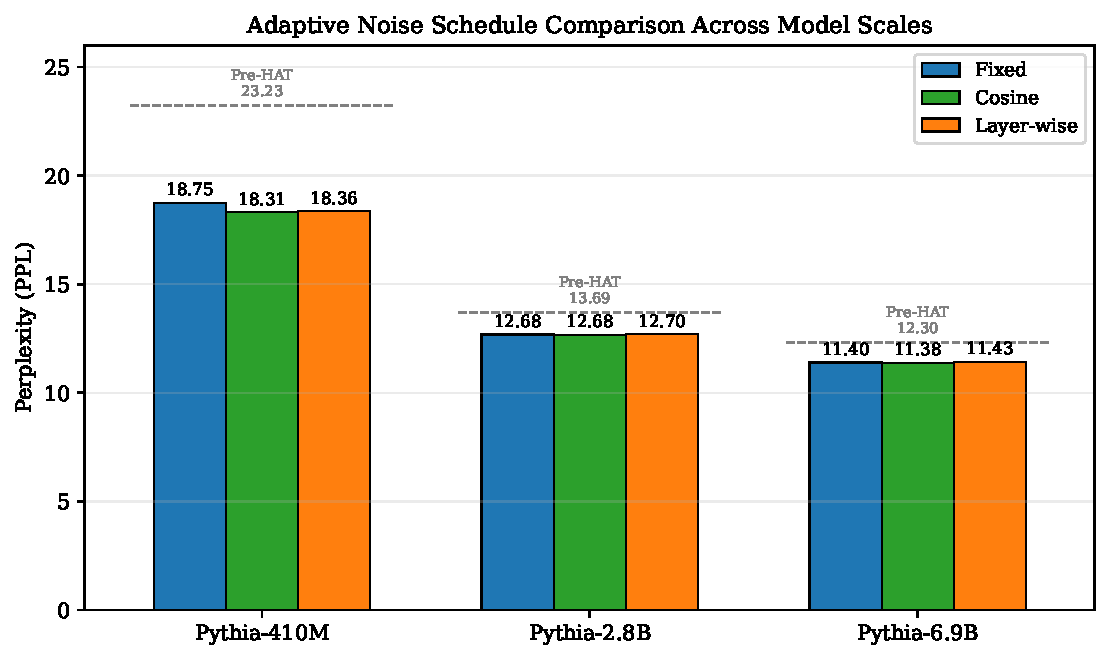
\includegraphics[width=0.88\textwidth]{../figures/remote107/fig_remote107_r3_adaptive_ppl_20260513.pdf}
\caption{Remote~107 R3自适应噪声调度比较。410M冻结目标层主线中，cosine decay达到最低PPL=18.31；reverse layer-wise退化到21.30，作为负面对照。2.8B和6.9B在fixed、cosine和layer-wise之间仅呈现小幅差异。}
\label{fig:remote107_r3_adaptive}
\end{figure}

真正出现结构性收益的是更大模拟覆盖范围的情形。图~\ref{fig:remote107_r3_p28b_ablation}给出了p28b的层范围与调度联合消融：last1 fixed为12.68，last1 cosine为12.68，last2 fixed为13.78，而last2+cosine进一步降至12.56，成为当前p28b路线中的最佳结果；last4 fixed则回升至14.12。这一结果说明，当模拟KV范围从单一终端层扩展到last2时，自适应调度可以弥补额外层引入的噪声敏感性，使last2路线重新回到可接受窗口。换言之，R3并没有推翻“last1是默认主路线”的判断，而是补充了一条更细的工程结论：若需要扩大模拟覆盖范围以换取更高面积或能效收益，优先考虑\texttt{last2+cosine}，而不是简单沿用fixed schedule。

\begin{figure}[htbp]
\centering
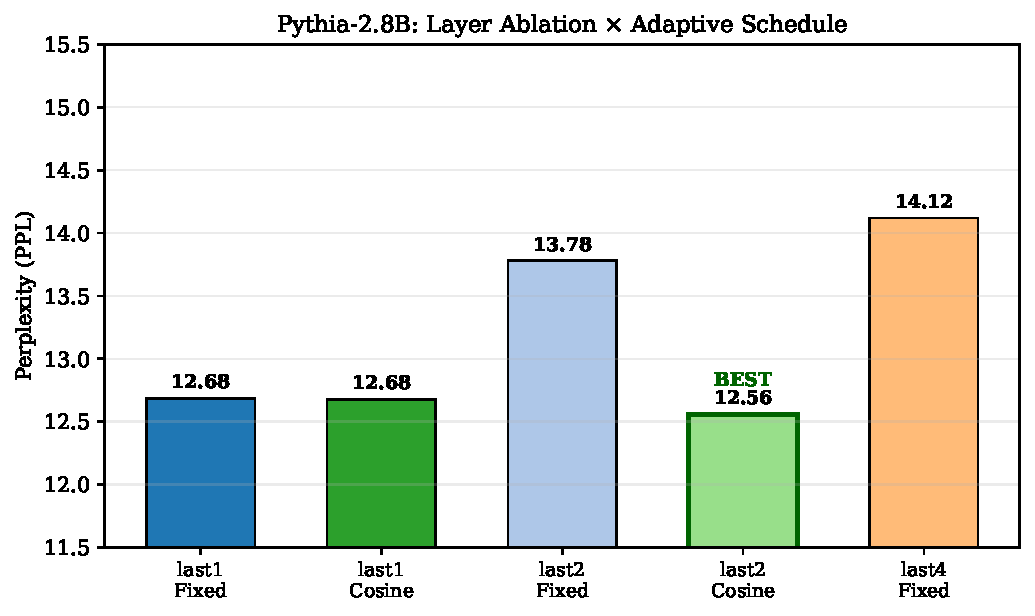
\includegraphics[width=0.82\textwidth]{../figures/remote107/fig_remote107_r3_p28b_ablation_20260513.pdf}
\caption{Pythia-2.8B层范围与调度联合消融。\texttt{last2+cosine}达到最佳PPL=12.56，优于\texttt{last2+fixed}的13.78，也略优于\texttt{last1+fixed}的12.68。}
\label{fig:remote107_r3_p28b_ablation}
\end{figure}

\textbf{证据边界说明}：p28b的checkpoint SHA256已修复为非空值，但仍需本地source-data packaging及manifest/SHA验证后方可升级为claim-bearing证据；p69b的checkpoint SHA256仍为null，当前仅作为provisional支持数据，不能独立支撑部署声明。


\section{预期贡献与创新点}
\label{sec:work2_contributions}

基于前述问题定义与实验设计，本工作预期在以下四个方面作出贡献。这些贡献既包括\textbf{知识增量}（对领域内尚未解答的问题给出新的认知），也包括\textbf{方法论增量}（为后续研究提供可复用的分析框架和工具链）。

第一，现有CIM-for-LLM研究集中于氧化物RRAM或SRAM器件，缺乏对有机光电CIM在该场景下的系统性评估。本工作将提供从器件噪声模型、保持时间衰减到注意力精度退化、下游任务性能的端到端基准测试，填补该领域的知识空白。该基准不仅服务于有机CIM社区，也为更广泛的"新兴存储技术$\rightarrow$LLM推理负载"映射研究提供了方法论模板。

第二，本工作将形式化论证有机OEC-RAM的$\sim$$10^3$ s保持时间与LLM边缘推理会话长度（秒至分钟级）的物理匹配性。这一论证并非简单的数值比较，而是通过多尺度建模（器件衰减模型$\rightarrow$电导漂移$\rightarrow$注意力分数偏移$\rightarrow$任务性能退化）建立的因果链条，为"何种存储技术适用于何种负载"这一普适问题提供方法论范例。该论证框架可推广至其他新兴存储技术（如FeFET、PCM、MRAM）的负载匹配分析，具有超越本工作具体场景的普适价值。

第三，本工作将系统评估光学刷新在KV缓存管理中的能效优势，量化其相对于电学刷新的耐久预算节省和能量节省。这一分析将修正Work 1中对有机光敏特性的悲观判断，展示同一物理特性在不同应用语境下可从"噪声源"转化为"系统优势"。实验四将输出"刷新间隔—任务准确率—总能量"的三维帕累托面，明确标识光学刷新可操作的设计空间，为后续有机CIM芯片的刷新控制器设计提供定量依据。

第四，通过实验三（压缩协同设计）和实验四（层级化刷新策略），本工作将提出"器件物理—量化编码—系统策略"的三层次协同设计框架，为后续有机CIM在边缘LLM推理中的工程实现提供可操作的优化空间。该框架的核心思想是：器件层的参数（$\tau$、$\sigma$、$N$）不是固定的约束，而是可与算法层（码本设计、注意力变体）和系统层（刷新策略、存储层级）联合优化的设计变量。这一思想打破了传统"器件先行、系统适配"的线性设计范式，体现了新兴计算范式所要求的\textbf{跨层次协同优化}理念。

这些贡献与Work 1形成明确互补。Work 1（第\ref{chap:hat-instance-overfitting}章）指出了有机CIM在ViT注意力推理中的结构性瓶颈：严重非线性叠加推理阶段的动态激活导致模拟精度快速退化。Work 2则转向\textbf{互补场景}——KV缓存的静态存储与WORM访问模式——探索有机CIM可能具备潜在优势的应用边界。两者共享同一行为级模拟器基础设施，但在科学结论上形成"证伪与假设生成"的互补结构，增强了硕士论文的理论完整性与论证深度。

Work 1的结论可概括为"有机CIM不适合需要高频动态激活更新的在线推理任务"，而Work 2的结论预期为"有机CIM适合需要低频写入、高频读取的静态存储任务"。这一对偶结论并非相互矛盾，而是共同界定了有机CIM的能力边界：其优势场景是那些能够利用其保持时间—耐久性最优区间、且规避其写入速度慢和循环变异大的负载。KV缓存正是这一优势场景的典型代表。


\section{范围边界与明确排除项}
\label{sec:work2_boundaries}

为确保研究的可控性和结论的严谨性，以下事项被明确排除在本工作当前范围之外。这些排除项并非因技术不可行而回避，而是基于资源约束和研究焦点的主动界定。

\begin{table}[htbp]
\centering
\caption{范围边界与排除理由}
\label{tab:boundaries}
\begin{tabular}{lp{8cm}}
\toprule
排除项 & 理由 \\
\midrule
>7B参数模型 & 有机交叉阵列的当前密度不足以单片容纳7B+模型的完整KV缓存；多片划分属于系统架构问题，非本工作的器件物理焦点 \\
>32k token上下文 & 超长上下文需要3D堆叠、混合存储层级或片外卸载，这些属于通用存储系统研究，不特定于有机CIM的物理贡献 \\
KV缓存的片上训练 & 训练过程需要高频原地更新K/V张量，超出有机器件$10^3$–$10^4$次耐久极限；该方向归入第\ref{ch:outlook}章展望（ continual learning 场景） \\
生产部署声明 & 本工作以行为级仿真为主，所有结论均标注"仿真验证"或"原型级"，不做大规模商用部署承诺 \\
完整光电协同设计 & 光子前端（photodiode）与CIM权重的联合训练属于Direction D的研究范畴，其部分洞察将汇入前端设计相关章节，但不作为独立实验展开 \\
多片/芯粒扩展 & 多片互连和芯粒（chiplet）架构属于Direction A的研究范畴，其部分设计考虑将汇入第\ref{sec:exp2_arch}节架构探索，但不作为独立贡献 \\
\bottomrule
\end{tabular}
\end{table}

明确的范围边界不仅是项目管理工具，更是学术严谨性的体现。在新兴器件研究中，常见的一类批评是"过度声称"（overclaiming）：将仿真或单器件结果不恰当地推广至远超其验证范围的系统场景。本工作通过主动界定边界，将结论的适用范围限制在"1–3B参数边缘LLM、4k–8k上下文、仿真验证级别、以KV缓存静态存储与读取为主要访问模式"之内。任何超出此范围的推广——如"有机CIM适用于所有LLM推理场景"——均被明确排除。

此外，边界界定有助于区分\textbf{本征贡献}与\textbf{工程外延}。本工作的本征贡献在于建立"有机CIM物理特性—KV缓存访问模式—系统性能指标"的映射关系；而7B+模型的多片扩展、128k上下文的3D堆叠、光电前端的联合优化等，均属于该本征贡献之上的工程外延，留待后续研究或产业界探索。这种区分使得本工作的科学焦点清晰，避免了因追求"全栈覆盖"而导致的论证稀释。

从学位论文的完成可行性角度，上述边界确保了研究工作量与硕士研究生培养周期的匹配。四组实验（噪声鲁棒性、架构探索、压缩协同设计、时间动态）的总仿真时间预计为200--400 GPU小时，在单卡RTX 5070 Ti上可于数周内完成。排除>7B模型和超长上下文后，单次实验的反馈周期控制在分钟级，支持充分的参数扫描和消融分析。若纳入7B模型或128k上下文，单次推理即可能耗时数小时，参数扫描将不可行。因此，范围边界的设定既是科学判断，也是对硕士论文实际可完成性的审慎评估。


\section{本章小结与向第七章的过渡}
\label{sec:work2_summary}

本章系统界定了硕士论文第二个核心工作（Work 2）的研究范围：以有机光电模拟存内计算（CIM）作为大语言模型KV缓存的存储与计算层，面向1–3B边缘LLM推理场景，通过行为级仿真评估有机CIM在物理特性上与KV缓存访问模式的结构性匹配。

本章的核心论点可概括为三个层次：\textbf{物理匹配}——有机OEC-RAM的$\sim$$10^3$ s保持时间和$10^3$–$10^4$次耐久性落入KV缓存WORM访问模式的"最优区间"；\textbf{机制优势}——光学刷新将Work 1中识别的"光敏噪声源"转化为低能耗、无耐久代价的数据维持机制；\textbf{系统评估}——Remote 107早期实验排除了全层模拟KV缓存作为主路线，后续selective-KV claim-lock packet在Pythia-410M、WikiText-2 raw-v1 test、context 512、non-overlapping stride 512、batch size 1下完成41/41个逐行JSON artifact归档：数字基线为PPL=23.30，last1/last2在D2D=0.02--0.05下保持在约18.6--19.0 PPL，而全层all24在D2D=0.05时恶化到$59.055\pm1.610$ PPL。该证据支持选择性终端层作为有机CIM KV缓存的主候选路线，全层模拟KV缓存仅保留为负面对照。

在方法论上，本工作沿用并扩展了Work 1建立的行为级模拟器框架，确保跨工作的一致性；在论证结构上，Work 2与Work 1形成互补——前者分析有机CIM在动态推理中的局限，后者论证其在静态存储中的优势，共同构建起"有机CIM适用性评估"的完整图景。

在结束本章之前，有必要基于Remote 107已获得的claim-lock数据明确Work 2的当前证据边界。当前证据支持假设~\ref{hyp:precision}在选择性终端层范围内作为主候选方向：last1/last2配置在$\sigma_{\text{d2d}} \leq 0.05$、8-bit量化条件下保持低困惑度和低跨种子方差；all24则在相同D2D窗口内快速恶化，因而只适合作为负面对照。这表明有机CIM KV缓存在特定层范围内具有进一步实验价值，但仍不构成生产部署声明。后续工作将关注：（1）长上下文与真实cache-path协议下的保持/刷新困惑度曲线；（2）last2及更大覆盖范围的HAT适配效益评估；（3）器件工艺优化（提升$\tau$和$N$）与光电前端集成。假设~\ref{hyp:retention}和~\ref{hyp:endurance}的验证尚需时间动态、能耗和刷新预算数据。

第七章将补充展开实验二（架构探索）的帕累托前沿分析、实验三（压缩协同设计）的有机模拟存储与KIVI数字量化对比、以及实验四（时间动态）的保持时间—刷新策略权衡曲线。实验一的阶段性趋势——全层模拟KV缓存的噪声敏感性、选择性终端层的候选可行性、以及last1/last2的fresh-D2D低敏感性——已在本章第\ref{sec:work2_results}节报告，第七章将不再重复，而是关注：（1）等footprint下有机模拟与数字量化的精度—能效对比；（2）延迟—能耗—面积三维空间中的最优配置识别；（3）时间动态条件下光学刷新的能效优势量化。各节均以FP16基线为参照，以$\Delta_{\text{PPL}}$和下游任务指标为统一比较语言，确保结论的可追溯性和可复现性。

第七章将在综合现有实验证据的基础上，对第\ref{sec:work2_problem}节提出的三项核心假设进行阶段性判断：假设\ref{hyp:retention}（保持时间匹配）和假设\ref{hyp:endurance}（耐久性适配）是否获得当前器件物理与时间动态数据的支持？假设\ref{hyp:precision}（模拟精度充分）是否在last1/last2选择性终端层范围内以$N$-$\sigma$操作窗口的形式成立？这些判断将限定或修正本章提出的中心论点，并为第八章的未来展望提供实证基础。
